\documentclass[a4paper,english]{report}

% Language and font encoding
\usepackage[utf8]{inputenc}
\usepackage[T1]{fontenc}
\usepackage[english,ngerman]{babel}

% Special characters
\usepackage{eurosym, tipa, textcomp, textgreek, upgreek}

% Mathematical symbols
\usepackage{amssymb, amsfonts, amsmath, dsfont}

% References and URLs
\usepackage[hidelinks]{hyperref}
\usepackage{cleveref}

% Images
\usepackage{graphicx} 
\usepackage{float} 
\graphicspath{graphics/}

% Text color
\usepackage[usenames,dvipsnames]{xcolor}

% Multiple captions in one figure
\usepackage{subcaption}

% Compact lists
\usepackage{paralist}

% Tables
\usepackage{longtable, array, tabularx, booktabs, colortbl}

% ToDos
\usepackage{todonotes}
\usepackage{changes}

% Source code listings
\usepackage{listings}

% Quotes (\enquote)
\usepackage[autostyle,autopunct=false]{csquotes}

% Icons
\usepackage{fontawesome5}

% Literature
\usepackage{natbib}

% Tracking changes
\usepackage{changes}
\definechangesauthor[color=blue, name={Christian}]{C}
\definechangesauthor[color=purple, name={Florian}]{F}

% Custom commands

% Acronyms
% ========
% The argument appears in small caps.
\newcommand\acro[1]{\textsc{\lowercase{#1}}}

% Variables
% =========
\newcommand\widefiguremargin{-.22\textwidth}
\newcommand\widefigurewidth{.49\textwidth}
\newcommand\widefiguregap{.02\textwidth}
\newcommand\widefiguresum{1.4\textwidth}

% Fachschaft logo
% ===============
\newcommand*{\fslogo}{\raisebox{+1.25ex}{
\includegraphics[height=6cm]{graphics/logo-fachschaft}}}

% Wide box
% ========
% Box that runs into both margins. To be used inside a floating environment like figure or table.
\newcommand\widebox[1]{
	\hspace{\widefiguremargin}
	\begin{minipage}{\widefiguresum}
		#1
	\end{minipage}
}

% Column rules
% ============
% Adds two rules each spanning approximately half of the available textwidth (as defined by \widefigurewidth).
\newcommand\colrules{
	\rule{\widefigurewidth}{0.4pt}
	\hspace{\widefiguregap}
	\rule{\widefigurewidth}{0.4pt}
}

% Simple code examples
% ====================
% Box for example code next to the rendered example.
%
% Arguments:
% 1. Label.
% 2. Content path without extension. If a corresponding PDF file exists, it gets included as an image. Otherwise, the LaTeX code gets rendered directly.
% 3. Caption.
\newcommand\example[3]{
	\Example{#1}{#2}{#2}{#3}
}

% Extended code examples
% ======================
% Box for example code next to the rendered example.
% Depending on the third argument, the source path for the right-side rendering can differ from the source path of the left-side listing.
% Useful if only an excerpt of the document to be rendered affects the entire output.
%
% Arguments:
% 1. Label.
% 2. Content path without extension. If a corresponding PDF file exists, it gets included as an image. Otherwise, the LaTeX code gets rendered directly.
% 3. Alternative path for Rendering (c.f. 2.)
% 4. Caption.
\newcommand\Example[4]{
	\begin{figure}[htp]
		\widebox{
			% Top rules:
			\colrules
			% Left content: code listing:
			\begin{subfigure}{\widefigurewidth}
				\inputminted[breaklines]{tex}{listings/#2.tex}
			\end{subfigure}
			\hspace{\widefiguregap}
			% Right content: image or rendered example:
			\begin{subfigure}{\widefigurewidth}
				\IfFileExists{listings/#3.pdf}{
					\includegraphics[width=\linewidth]{listings/#3.pdf}
				}{
					\medskip
					\input{listings/#3}
					\medskip
				}
			\end{subfigure}
			% Bottom rules:
			\colrules
			% Left caption:
			\begin{subfigure}[t]{\widefigurewidth}
				\caption{\LaTeX-Code}
				\label{#1-code}
			\end{subfigure}
			\hspace{\widefiguregap}
			% Right caption:
			\begin{subfigure}[t]{\widefigurewidth}
				\caption{Ergebnis}
				\label{#1-result}
			\end{subfigure}
		}
		% General caption:
		\caption{#4}
		\label{#1}
	\end{figure}
}

% Exercise mode
% =============
% The exercise mode can be chosen by writing one of the following to the exercise-mode.tex file before compilation:
% \newcommand\exercisemode{none}      % for a blank script without exercises
% \newcommand\exercisemode{exercises} % for a script with exercises only
% \newcommand\exercisemode{solutions} % for a script with solutions only
% \newcommand\exercisemode{any}       % for a script containing all available material
% The following lines include that file or make \exercisemode default to 'any' so that any derivatives of this project will work even without the file.
\IfFileExists{exercise-mode.tex}{
	\input{exercise-mode.tex}
}{
	\newcommand\exercisemode{any}
}

% Exercises
% =========
% Includes the task.tex file within the given subfolder of exercises and adds a heading.
\newcommand\exercise[1]{
	\ifthenelse{\equal{\exercisemode}{none}}{
		% Exercises disabled.
	}{
		\newpage
		\definecolor{latexblue}{rgb}{0.9,0.925,0.95}
		\pagecolor{latexblue}
		%\definecolor{latexblue}{rgb}{0.73,0.84,0.92}
		\section*{Exercise \thechapter}
		\addcontentsline{toc}{section}{Übung}%
		The following list shows some key data about a few courses of the \acro{WIAI} faculty.
However, the overview is not as clear as it could be.
To improve it, convert the list into a table with columns for \emph{name}, \emph{abbreviation} and \emph{term}.
Insert an additional \emph{centered column} that numbers the courses. 
Add a caption to the table.
You find the table in \mintinline{bash}{exercises/tables/tables.tex}.

\todo{Beispieldaten übersetzen?}
\exercisematerial{exercises/tables/tables}



		\newpage
		\nopagecolor
	}
}

% Exercise Material
% =================
% Takes a project-relative path, and inserts matching exercise material and/or solutions, depending on the exercise mode.
\newcommand\exercisematerial[1]{
	% Mode 'exercises': raw material only
	\ifthenelse{\equal{\exercisemode}{exercises}}{
		\IfFileExists{#1.raw.tex}{
			\input{#1.raw.tex}
		}{}
	}{}
	% Mode 'solutions': completed material only
	\ifthenelse{\equal{\exercisemode}{solutions}}{
		\IfFileExists{#1.done.tex}{
			\input{#1.done.tex}
		}{}
	}{}
	% Mode 'any': all existing material. If both raw and completed material exist, headings are added for each.
	\ifthenelse{\equal{\exercisemode}{any}}{
		\IfFileExists{#1.raw.tex}{
			\IfFileExists{#1.done.tex}{
				\subsubsection*{Vorschau des ungelösten Materials}
			}{}
			\input{#1.raw.tex}
		}{}
		\IfFileExists{#1.done.tex}{
			\IfFileExists{#1.raw.tex}{
				\subsubsection*{Vorschau des gelösten Materials}
			}{}
			\input{#1.done.tex}
		}{}
	}{}
}



% Optional: Minted for source code listings
\ifthenelse{\equal{\listingsmode}{minted}}{%
  \usepackage{minted}
}{} % Preamble

% Acronyms
% ========
% The argument appears in small caps.
\newcommand\acro[1]{\textsc{\lowercase{#1}}}

% Variables
% =========
\newcommand\widefiguremargin{-.22\textwidth}
\newcommand\widefigurewidth{.49\textwidth}
\newcommand\widefiguregap{.02\textwidth}
\newcommand\widefiguresum{1.4\textwidth}

% Fachschaft logo
% ===============
\newcommand*{\fslogo}{\raisebox{+1.25ex}{
\includegraphics[height=6cm]{graphics/logo-fachschaft}}}

% Wide box
% ========
% Box that runs into both margins. To be used inside a floating environment like figure or table.
\newcommand\widebox[1]{
	\hspace{\widefiguremargin}
	\begin{minipage}{\widefiguresum}
		#1
	\end{minipage}
}

% Column rules
% ============
% Adds two rules each spanning approximately half of the available textwidth (as defined by \widefigurewidth).
\newcommand\colrules{
	\rule{\widefigurewidth}{0.4pt}
	\hspace{\widefiguregap}
	\rule{\widefigurewidth}{0.4pt}
}

% Simple code examples
% ====================
% Box for example code next to the rendered example.
%
% Arguments:
% 1. Label.
% 2. Content path without extension. If a corresponding PDF file exists, it gets included as an image. Otherwise, the LaTeX code gets rendered directly.
% 3. Caption.
\newcommand\example[3]{
	\Example{#1}{#2}{#2}{#3}
}

% Extended code examples
% ======================
% Box for example code next to the rendered example.
% Depending on the third argument, the source path for the right-side rendering can differ from the source path of the left-side listing.
% Useful if only an excerpt of the document to be rendered affects the entire output.
%
% Arguments:
% 1. Label.
% 2. Content path without extension. If a corresponding PDF file exists, it gets included as an image. Otherwise, the LaTeX code gets rendered directly.
% 3. Alternative path for Rendering (c.f. 2.)
% 4. Caption.
\newcommand\Example[4]{
	\begin{figure}[htp]
		\widebox{
			% Top rules:
			\colrules
			% Left content: code listing:
			\begin{subfigure}{\widefigurewidth}
				\inputminted[breaklines]{tex}{listings/#2.tex}
			\end{subfigure}
			\hspace{\widefiguregap}
			% Right content: image or rendered example:
			\begin{subfigure}{\widefigurewidth}
				\IfFileExists{listings/#3.pdf}{
					\includegraphics[width=\linewidth]{listings/#3.pdf}
				}{
					\medskip
					\input{listings/#3}
					\medskip
				}
			\end{subfigure}
			% Bottom rules:
			\colrules
			% Left caption:
			\begin{subfigure}[t]{\widefigurewidth}
				\caption{\LaTeX-Code}
				\label{#1-code}
			\end{subfigure}
			\hspace{\widefiguregap}
			% Right caption:
			\begin{subfigure}[t]{\widefigurewidth}
				\caption{Ergebnis}
				\label{#1-result}
			\end{subfigure}
		}
		% General caption:
		\caption{#4}
		\label{#1}
	\end{figure}
}

% Exercise mode
% =============
% The exercise mode can be chosen by writing one of the following to the exercise-mode.tex file before compilation:
% \newcommand\exercisemode{none}      % for a blank script without exercises
% \newcommand\exercisemode{exercises} % for a script with exercises only
% \newcommand\exercisemode{solutions} % for a script with solutions only
% \newcommand\exercisemode{any}       % for a script containing all available material
% The following lines include that file or make \exercisemode default to 'any' so that any derivatives of this project will work even without the file.
\IfFileExists{exercise-mode.tex}{
	\input{exercise-mode.tex}
}{
	\newcommand\exercisemode{any}
}

% Exercises
% =========
% Includes the task.tex file within the given subfolder of exercises and adds a heading.
\newcommand\exercise[1]{
	\ifthenelse{\equal{\exercisemode}{none}}{
		% Exercises disabled.
	}{
		\newpage
		\definecolor{latexblue}{rgb}{0.9,0.925,0.95}
		\pagecolor{latexblue}
		%\definecolor{latexblue}{rgb}{0.73,0.84,0.92}
		\section*{Exercise \thechapter}
		\addcontentsline{toc}{section}{Übung}%
		The following list shows some key data about a few courses of the \acro{WIAI} faculty.
However, the overview is not as clear as it could be.
To improve it, convert the list into a table with columns for \emph{name}, \emph{abbreviation} and \emph{term}.
Insert an additional \emph{centered column} that numbers the courses. 
Add a caption to the table.
You find the table in \mintinline{bash}{exercises/tables/tables.tex}.

\todo{Beispieldaten übersetzen?}
\exercisematerial{exercises/tables/tables}



		\newpage
		\nopagecolor
	}
}

% Exercise Material
% =================
% Takes a project-relative path, and inserts matching exercise material and/or solutions, depending on the exercise mode.
\newcommand\exercisematerial[1]{
	% Mode 'exercises': raw material only
	\ifthenelse{\equal{\exercisemode}{exercises}}{
		\IfFileExists{#1.raw.tex}{
			\input{#1.raw.tex}
		}{}
	}{}
	% Mode 'solutions': completed material only
	\ifthenelse{\equal{\exercisemode}{solutions}}{
		\IfFileExists{#1.done.tex}{
			\input{#1.done.tex}
		}{}
	}{}
	% Mode 'any': all existing material. If both raw and completed material exist, headings are added for each.
	\ifthenelse{\equal{\exercisemode}{any}}{
		\IfFileExists{#1.raw.tex}{
			\IfFileExists{#1.done.tex}{
				\subsubsection*{Vorschau des ungelösten Materials}
			}{}
			\input{#1.raw.tex}
		}{}
		\IfFileExists{#1.done.tex}{
			\IfFileExists{#1.raw.tex}{
				\subsubsection*{Vorschau des gelösten Materials}
			}{}
			\input{#1.done.tex}
		}{}
	}{}
}

 % Custom commands
% \addbibresource{literature.bib}

\title{Skript zum \LaTeX-Tutorium der Fachschaft \acro{WIAI}}
\author{Evelyn Fradtschuk \and Florian Knoch \and Christian Kremitzl \and Bernhard Luedtke}

\begin{document}

% Title page
\thispagestyle{empty}
\begin{center}
	\fslogo \\
	\vspace{3em}
	\rule{\textwidth}{1pt}\par
	\vspace{0.8\baselineskip}
			\Huge\bfseries Script for the Fachschaft \acro{WIAI} \LaTeX{} Workshop
	\rule{\textwidth}{1pt}\par
	%{\large \today}
	\vfill
	\vfill
	{\Large{ Evelyn Fradtschuk, Florian Knoch,\\
	Christian Kremitzl, Bernhard Luedtke}}\\		
	\vfill
\end{center}

\newpage
\thispagestyle{empty}

\mbox{}
\vfill

\begin{tabular}{@{}lp{9cm}}
	& \subsubsection*{Imprint} \\
	& The \LaTeX{} Script (version 1.1 from October Xth, 2021) has been assembled by the Student Council of the Information Systems and Applied Computer Sciences Faculty (Fachschaft \acro{WIAI}) at the University of Bamberg. \\
	& It is licensed unter Creative Commons \enquote{Attribution-ShareAlike 4.0 International} (CC BY-SA 4.0): \\
	\href{http://creativecommons.org/licenses/by-sa/4.0/}{
\includegraphics[height=.5cm]{graphics/cc-by-sa}} & \url{http://creativecommons.org/licenses/by-sa/4.0/} \\ \\
	& Upon request, allowances exceeding the limitations of this license may be granted.
\end{tabular}

% or simply 
% \maketitle
\thispagestyle{empty}
\newpage

\setcounter{page}{1} % Don't count title page.
\setcounter{tocdepth}{2}
\tableofcontents
\newpage

\chapter{What is \LaTeX?}
\label{sec:what-is-latex}

In the early 1960s, a rather talented American Ph.D. student was asked by a big publishing company whether he wanted to write a book on compilers.
He did.
Soon after he had begun with his research, he realized that he wanted to start with some foundations of computer science, so he asked the publishers if the book might be a little longer.
They replied, \enquote{make it as long as you feel necessary.}
In 1968, the first volume was published, at that time still printed using mechanical typesetting.

This method was just disappearing then, and being replaced by new methods.
However, the author did not like the results of those new methods, so,
at the end of the 70s, he began to develop his own typesetting system \TeX{}
(pronounced as \emph{tech}\todo{is that a valid transliteration in english?}), named after the ancient Greek word \texttau$\mathrm{\acute{\varepsilon}}$\textchi\textnu\texteta{} (technē) meaning \emph{art, craft}.

Today, Donald Knuth (that is the former student’s name) is a retired professor of computer science and his compiler book has grown to become the multi-volume standard work \emph{The Art of Computer Programming}\,—\,three volumes of which are still to be written, among them the one on compilers.
Unlike the book, however, \TeX{} is the rare occurrence of a software system that may actually be called \emph{complete} without meaning \emph{dead}.

Two more letters are needed for \LaTeX:
They are the initial two letters of the last name of Leslie Lamport, who, in the 80s, extended \TeX{} by a collection of small programs that made the entire system usable for us end-users and are responsible for its widespread adoption.
The current version dates from the mid~90s.

Why are we telling you all of that?
It explains some of the advantages that still distinguish \LaTeX{} today:
It is a mature, stable, and reliable system
that does typesetting in a typographically sophisticated way and mostly automatically.

As the \TeX{} code is stored in plaintext files (cf. \cref{sec:basic-functionality}),
even more advantages arise:
You can structure your projects clearly (cf. \cref{sec:project-structure}),
and whenever you undo changes in the source code, you can always rely on getting exactly the same output as before.
\todo{Klingt für mich, als würden Undos nichts bewirken. (F)}
On a larger scale, this does also work in connection with Git or other source code versioning tools.
Furthermore, you can trust your source code to be readable long-term, without any specific software.
It can always be opened with any program that supports plaintext.
\todo{maybe, a heading like “Why use \LaTeX?” would better fit the content …}

% Quellen:
% https://en.wikipedia.org/wiki/Donald_Knuth
% https://de.wikipedia.org/wiki/Donald_E._Knuth
% https://en.wikipedia.org/wiki/The_Art_of_Computer_Programming
% https://de.wikipedia.org/wiki/The_Art_of_Computer_Programming
% https://en.wikipedia.org/wiki/TeX
% https://de.wikipedia.org/wiki/TeX
% https://de.wikipedia.org/wiki/LaTeX
% https://en.wikipedia.org/wiki/LaTeX


\chapter{How does \LaTeX{} function?}
\label{sec:basic-functionality}

\todo{Really ``function'', not ``work''?}
\todo{I’d prefer “work,” too.}

Word processing and document creation programs have to decide how to translate user input into a document layout.
There are different concepts to approach this topic.
When working with Microsoft Word, the rule is: a document exported as \acro{PDF} looks exactly like the source document in Word. 
Where a graphic is placed in Word, it is also found in the \acro{PDF}. 
Adjustments to the appearance in Word and other popular programs thus result in a direct visual change. 
This type of formatting is called \emph{What you see is what you get} (\acro{WYSIWYG} for short). 
Content and \replaced[id=C]{formatting}{structure} are closely linked.

\LaTeX{}, on the other hand, works according to the principle \emph{What you get is what you mean} (\acro{WYGIWYM} for short). 
Content and \replaced[id=C]{formatting}{structure} are separated more clearly.
The content is placed in a document in plain text form, together with so-called \emph{commands}. 
The combination of text content and commands is also called \emph{source} \replaced[id=C]{code}{text}.
\todo{Nicht source code?} 

To customize the presentation of the content, we do not change the text content itself but add appropriate commands instead. 
\todo{Vielleicht lieber Gegenüberstellung: Statt über eine GUI Styles zu vergeben, annotieren wir explizit mit Commands – und zwar hauptsächlich semantisch.}
These are processed by a \emph{compiler}, which adjusts the resulting appearance depending on the command. 
Line by line, the compiler processes text and commands from our source code. 
When all the source code has been processed by the compiler, we get the final document. 
There are different export options, but most of the time we output the document as a \acro{PDF}\,---\,just like in Word.

As a brief example for a command, we shall use the \replaced[id=C]{emphasis}{highlighting} of words or sentences. 
The command is \mintinline{latex}{\emph{}}. 
We write the text we want to \replaced[id=C]{emphasize}{highlight} inside the curly brackets in the source code, like this: 
\mintinline{latex}{\emph{Good morning!}}. 
In the resulting PDF, this text will appear in italics: \emph{Good morning!} 
There is no trace of the command identifier and the special characters. 
You can see, we are not writing italic text inside the source code, we just tell the compiler that certain words should be \replaced[id=C]{emphasized}{highlighted} by the use of a command.

This simple example illustrates a strength of the \acro{WYGIWYM} principle. 
We mark text elements on \replaced[id=C]{a}{the} semantic level and can make the associated typographic adjustments centrally\,---\,or let \LaTeX{} do the configuration itself.
For instance, if we want to change the way highlighting is done, we can configure this once. 
At all places where \mintinline{latex}{\emph{}} is used, the final result will be adjusted accordingly. 
There is no need to make adjustments at each occurrence of an emphasized word. 
The principle is similar to style sheets in office programs, although more consistent and powerful.

\section{What do we need to use \LaTeX{}?}
\label{subsec:what-we-need}

If we want to generate a PDF document with \LaTeX{}, we need at least two programs. 
One to create the source code, and a second to process the source code. 
The latter is the already mentioned compiler.

In principle, a simple text editing program is sufficient for creating the source code. 
Most\todo{Is there one that doesn’t?} operating systems provide such programs out of the box. 
Maybe you are already used to applications like Notepad++,\footnote{Available at \url{https://notepad-plus-plus.org/}.} these are usable as well. 
Then there are advanced programs like \TeX{}studio\footnote{Available at \url{https://www.texstudio.org/}.} or Texmaker\footnote{Available at \url{https://www.xm1math.net/texmaker/}.} which integrate additional functions that facilitate the use of commands.
You \replaced[id=C]{have free choice}{are free to choose}.
\todo{Hier nochmal, analog zum Vorwort, auf unsere Empfehlung verweisen?}

As mentioned before, we need a compiler to be able to compile our source code.
The compiler is usually part of a collection of \emph{programs} and \emph{packages} which are together called a \LaTeX-\emph{distribution}. 
The included packages provide various additional commands. 
For now, we will skip over the many programs.\footnote{We will get to know one of these helper programs later on, in \ref{sec:literature}, when we are citing literature.}

Multiple different \LaTeX{} distributions exist. 
Some of the well-known ones are MiK\TeX,\footnote{For Windows, macOS and Linux. Available at \url{https://miktex.org/}.} Mac\TeX,\footnote{For macOS and Linux. Available at \url{https://www.tug.org/mactex/}.} and \TeX{} Live.\footnote{For Windows, macOS, and Linux. Available at \url{https://www.tug.org/texlive/}.}\todo{Hier tobt ein Edit War … Fußnoten bitte immer *nach* Satzzeichen!}
It is best to install one of them right away. 
The installation may take several hours. 
For this reason, some distributions are available for download in a small and a full version. 
The full version contains all packages, while the small version downloads packages only when they are needed.
Unfortunately, we cannot take away the decision if you would rather wait for the download at the beginning or later while you are working.
\todo{Ich sehe entsetzte Gesichter von Leuten mit kleinen Festplatten, die glauben, sie brauchen alle Packages.}
\todo{:D Ich hätte gedacht, wir sollten vielleicht durchaus das Runterladen empfehlen, damit sie im Tut weniger warten müssen. Bringt aber den Windows-Leuten wohl eh nix}

\section{The commands}
\label{subsec:command-structure}
The commands used in source code follow a general structure:
\begin{minted}{xml}
\<command>[<optional_parameters>]{<mandatory_parameters>}
\end{minted}
A command can use several optional and/or mandatory parameters. 
Some commands have no mandatory parameters at all. 
Some examples are shown in \cref{tbl:latex-commands}.

\begin{table}[h!]
	\widebox{
		\begin{tabular}{@{}p{\widefigurewidth}p{\widefigurewidth}@{}}
			\toprule
			Command                                                  & Effect                             \\
			\midrule
			\mintinline{latex}{\newpage}                              & inserts a new page           \\
			\mintinline{latex}{\textbf{Text}}                         & prints the text in bold font \\
			\mintinline{latex}{\usepackage[utf8]{inputenc}}           & sets the text encoding to \acro{UTF-8}  \\
			\mintinline{latex}{\documentclass[a4paper,12pt]{article}} & specifies the document class  \\
			\mintinline{latex}{\frac{3}{4}}               & inserts a mathematical fraction  \\
			\bottomrule
		\end{tabular}
	}
	\caption{Examples for \LaTeX-commands}
	\label{tbl:latex-commands}
\end{table}

If a command allows multiple optional parameters that accept similar inputs, it is sometimes necessary to specify which parameter is meant. 
For example, the command for embedding graphics accepts optional parameters for width and height. 
If \mintinline{tex}|[12cm, 4cm]| were entered, it would be unclear which value is intended for which parameter. 
To make the assignment more concrete, \replaced[id=C]{it is possible to}{we can} specify the parameters explicitly:
\todo{Can or have to?}
\todo{Grundsätzlich can, aber es ist nicht unsere Entscheidung, deswegen würde ich das impersonal formulieren}
\begin{minted}{tex}
\includegraphics[width=12cm, height=4cm]{picture.png}
\end{minted}

As the examples already show, many different commands can be used. 
Some are intended for use in mathematical formulas, others allow the inclusion of graphics. 
In the beginning, it will take some getting used to. 
\todo{So klingt es vielleicht nicht ganz so bedrohlich …}
\replaced[id=C]{However, you don’t have to learn every single command by heart: As soon as you remember the most important commands, you can easily create simple documents and look up everything else.}{Remembering all the relevant commands is hard, but after some practice and patience, simple documents can be created in no time.}


\chapter{Basic document structure}
\label{sec:basic-document-structure}

In essence, every \LaTeX{} document is composed of two parts: 
We call the first commands within our \LaTeX{} document the \emph{preamble}.
It specifies global properties of our document, such as the document class, the encoding, the language, the page format, and additional packages that we want to use.
The \emph{document environment}, on the other hand, contains the actual content of our document, i.\,e., the things that we will later see in our generated \acro{PDF} file. 

\Example{lst:latex-document-basic-structure}{basic-document-structure/hello-world}{basic-document-structure/hello-world_crop}{Exemplary structure of a simple \LaTeX{} document with preamble and document environment}

\section{Preamble}
Let's take a closer look at the preamble. 
A minimal preamble should contain the following specifications: 

\subsection{Document class}\label{sec:document-class}
We can define a document class by using the command \code{latex}{\textbackslash documentclass[<para- meter>]\{<document class>\}}.
The most commonly used document classes that are supported by default are \pkg{article} for short documents, and \pkg{report} for longer ones. 
Furthermore, you can use \pkg{book} for books, \pkg{beamer}\footnote{We do not cover making presentations in \LaTeX{} in this tutorial. However, if you are interested in the topic, we recommend this introduction on Overleaf: \url{https://www.overleaf.com/learn/latex/Beamer}} for presentations, and \pkg{letter}\footnote{We also do not cover letters in this script. An introduction can be found on WikiBooks: \url{https://en.wikibooks.org/wiki/LaTeX/Letters}} for letters.

In addition to the standard document classes, the \acro{KOMA} script classes have been developed. 
They provide alternatives to the document classes mentioned above: 
In lieu of \pkg{article} you can use \pkg{scrartcl}, \pkg{report} is replaced by \pkg{scrreprt},\footnote{Those vowels are indeed missing, do not try to insert them.} and \pkg{scrbook} can be used instead of \pkg{book}. 
As a replacement for \pkg{letter}, one can use \pkg{scrlttr2}. 
A complete list of all \acro{KOMA} script classes is available online.\footnote{Available at: \url{https://komascript.de/komascriptbestandteile}} 
By using \acro{KOMA} document classes, the layout of the generated \acro{PDF} document is changed. 
On top of that, they provide additional functionalities. 
The standard document classes are designed according to US-American conventions
whereas \acro{KOMA} classes adhere to European norms, e.\,g., for 
writing letters. 

Each \code{latex}{\textbackslash documentclass} command can hold optional parameters in 
square brackets. 
\code{latex}{\textbackslash documentclass[10pt,a5paper,landscape]scrartcl\}}, 
for instance, configures a \acro{KOMA} script article and sets its font size to 
10\,pt,\footnote{The standard font size is 12\,pt.} the page size to 
A5,\footnote{The default case would be A4.} and the orientation of the page to 
landscape. 
The language can be passed as an optional parameter, too (cf. \cref{sec:language}). 

\subsection{Digression: packages}
\label{sec:packages}

\codeblock{latex}{listings/basic-document-structure/packages.tex}
Packages provide additional commands and functionalities that we can use within our \LaTeX{} source code. 
There are numerous packages for different use cases (e.\,g., typesetting formulas, lists, \textellipsis). 
In order to use a package, it must be included within the preamble. 
To do so, the above-mentioned command is used. 
The most important \LaTeX{} packages can be found in the Comprehensive \TeX\ Archive Network, short: \acro{CTAN}.\footnote{Available at: \url{https://www.ctan.org/}} 
You can also find documentation for the packages there. 

\subsection{Encoding}
\codeblock{latex}{listings/basic-document-structure/encoding.tex}
One use case for packages is specifying the encoding of our \LaTeX{} document. 
The character encoding\footnote{cf. \url{https://en.wikipedia.org/wiki/Character_encoding}} determines the available character set.
The standard encoding in \LaTeX{} is \acro{ASCII}.\footnote{cf. \url{https://en.wikipedia.org/wiki/ASCII}}
It is an American character encoding and therefore does not contain German umlauts or most other special characters, which makes it unsuitable at least for non-english use cases. 
Instead, \acro{UTF-8}\footnote{cf. \url{https://en.wikipedia.org/wiki/UTF-8}} can be used as a universal character encoding.

In \LaTeX{}, we need to specify two character encodings: 
The input encoding (\mono{inputenc}), which refers to our source code, and the font encoding (\mono{fontenc}), which determines what the content of our \acro{PDF} document looks like.\footnote{Details on \mono{fontenc} can be found at: \url{https://tex.stackexchange.com/questions/108417/font-encoding-in-latex}}
\pkg{T1} is an encoding that tries to cover most European languages with a limited number of characters. 

\subsection{Language}\label{sec:language}
\codeblock{latex}{listings/basic-document-structure/language.tex}
The package \pkg{babel} provides language-specific information (e.\,g., on hyphenation, special characters, changing fonts, translation of labels\footnote{cf. \cref{sec:references}} like \enquote{Chapter,} \enquote{Table of Contents,} or \enquote{Figure.}
The desired language can be passed as an optional parameter. 
\pkg{ngerman}, for instance, is used for the new German spelling. 
Some packages require that the language is already passed as an optional parameter in the \code{latex}{\textbackslash documentclass} command. 
In this case, just leave out the optional parameter for the language within the \pkg{babel} inclusion command.

We can also use multiple languages in our document. 
To do so, we pass the languages, separated by commas, as an optional parameter to the babel inclusion command. 
Within our document, we can switch between languages with the \code{latex}{\textbackslash selectlanguage\{<language>\}} command. 
Alternatively, foreign-language text can be declared by using the following command: 

\codeblock{latex}{listings/basic-document-structure/foreign-language.tex}

\section{Document environment}
The actual content of the \acro{PDF} document needs to be put between \code{latex}{\textbackslash begin\{document\}} and \code{latex}{\textbackslash end\{document\}}.

\subsection{Continuous text}
The easiest content that we can integrate into the document environment is continuous text. 
We can write it directly into our source code. 
Line breaks and multiple consecutive spaces are ignored by \LaTeX{}. 
Blank lines create a new paragraph, that is indented by default.\footnote{The automatic indentation of new paragraphs can be prevented by using the command \code{latex}{\textbackslash noindent}.}
Manual line breaks can be enforced with two backslashes (\textbackslash\textbackslash). 
This should be avoided, though. 

\subsection{Comments}
Some characters are reserved for \LaTeX-specific commands, for instance, the percent sign. 
Using a percent sign tells the \LaTeX{} compiler to ignore the rest of the line, so the text after the percent character will not appear in the generated \acro{PDF} document.
This is called a \emph{comment}\textit{,}
and it can be useful to take notes while working on a document without affecting the document itself. 

There are a few more of these reserved characters, as we will see and learn to deal with in \cref{sec:more-special-characters}.

\subsection{Sections and chapters}
Continuous text can be structured by headings that divide the document into sections and chapters. 
Needless to say, \LaTeX{} provides us with commands for that.
The commands that are depicted in \cref{lst:headlines} can be used with any document class. 

\Example{lst:headlines}{basic-document-structure/headlines}{basic-document-structure/headlines_crop}{Heading Levels}

Some document classes provide additional commands. In a \pkg{report}, you get \code{late}{\textbackslash chapter\{Chapter\}}, and in a \pkg{book}, additionally \code{latex}{\textbackslash part\{Part\}}.
You can mark the command with an asterisk if you want to omit the numbering of a section and exclude it from the table of contents:\footnote{cf. \cref{sec:table-of-contents}}

\codeblock{latex}{listings/basic-document-structure/section.tex}

An alternative title for the table of contents can be declared as an optional 
parameter in square brackets between the command and the actual title:

\codeblock{latex}{listings/basic-document-structure/title-in-toc.tex}

\subsection{Front matter}
A simple front matter can be created by using the command \code{latex}{\textbackslash maketitle}. 
The values to be inserted into the front matter must be specified within the preamble. 
Multiple authors are joined by \code{latex}{\textbackslash and}.
If the date is not specified by the \code{latex}{\textbackslash date} command, the current date will be inserted by default.
The design of the front matter depends on the specified document class.

\Example{lst:titles}{basic-document-structure/titles}{basic-document-structure/titles_crop}{The front matter}

\subsection{Indices}\label{sec:table-of-contents}

The command \code{latex}{\textbackslash tableofcontents} generates an automatically numbered table of contents by making use of the above-mentioned commands for dividing our text into sections and chapters (this can bee seen in \cref{lst:main-file} on \cpageref{lst:main-file}).

The numbering style and depth, and many other options can, of course, be specified manually.\footnote{We recommend the following blogpost: \url{https://texblog.org/2011/09/09/10-ways-to-customize-tocloflot/}}
For \LaTeX{} to create our table of contents properly, the project has to be compiled twice.

Besides the table of contents, you can also generate a \code{latex}{\textbackslash listoffigures} (list of figures) and a \code{latex}{\textbackslash listoftables} (list of tables). 
The captions of your figures and tables will appear within those indices.\footnote{cf. \cref{sec:graphics} (Graphics) and \cref{sec:tables} (Tables) for more information on captions}

\exercise{basic-document-structure}
\chapter{Project structure}
\label{sec:project-structure}

In the previous chapters, we have only seen very short \LaTeX{} examples. \LaTeX{} can of course also be used to create larger documents and projects, such as a thesis. 
In order not to lose the overview in the source code and to avoid that source files become too long, a reasonable structuring of a larger \LaTeX{} project is advisable. For this purpose, the source code is divided into different files, which will be discussed in more detail in the following sections.

\section{Main file}

In large projects, we typically use one main file, which is often called \file{main.tex}. It is, in a sense, the structural skeleton of the project, as it contains the basic structure including the preamble. The title, table of contents, as well as the individual chapters of a work are integrated in this main file (cf.\ \cref{lst:main-file}). The inclusion of the individual sections can be done either by \code{latex}{\textbackslash input\{...\}} or \code{latex}{\textbackslash include\{\textellipsis\}}. Both require the path to the file to be included as an argument. We will discuss the differences between the two commands later (see \cref{sec:input-vs-include}).

\example{lst:main-file}{project-structure/main-file}{Typical structure in a main file \LaTeX{}}

\section{Section files}
Section files are files that are included within the main file. In a thesis, for example, these can be individual chapters. You are free to decide how granular the division of the content into individual files should be.
The files that are included by the main file do not contain a preamble, since this is already present in the main file. Neither do the commands \code{latex}{\textbackslash begin\{document\}} and \code{latex}{\textbackslash end\{document\}} appear again.

\section{Input or include?}
\label{sec:input-vs-include}

Let us now turn to the differences between the two possible commands for including \LaTeX{} files. Briefly summarized, \code{latex}{\textbackslash include} and \code{latex}{\textbackslash input} have differences in the following three aspects: The way in which the path to the file to be included is specified, the possibility of nesting inclusions, and whether a new page is started for each section.

If you use the command \code{latex}{\textbackslash input}, you can specify the file extension \mono{.tex}, but it is not mandatory. It is also possible to nest the inclusion of files: A file included with \code{latex}{\textbackslash input} can in turn include another file with the same command. The files that have been included are inserted in the finished document without starting a new page for the included section (cf. \cref{lst:main-file}).

The command \code{latex}{\textbackslash include} behaves differently: Here, the file 
extension \mono{.tex} \emph{must} be omitted. Nesting of embeddings is not 
possible. Also, a new page is created for each included file.

\chapter{Special characters}

\label{sec:special-characters}

\section{Spaces}

The special character used most frequently is a simple space between words.
\LaTeX{} creates it whenever the source code contains spaces or single newlines (by hitting the enter key once) between other characters.
The word space is not the only one, though\,---\,there are a few more types of spaces.
\Cref{lst:spaces} illustrates how they are used.

\example{lst:spaces}{special-characters/spaces}{Different spaces in \LaTeX}

\paragraph{English Spacing}
In documents written in English, \LaTeX{} uses traditional English Spacing by default. That is, double spaces after each sentence.
We can prevent this by using the command \code{tex}{\textbackslash frenchspacing} above the first paragraph.
With \code{latex}{\textbackslash nonfrenchspacing}, we can reset the behavior.
When using English Spacing, \LaTeX{} tries to recognize abbreviations and to use normal spaces after those.
We should still check this and\,---\,where necessary\,---\,enforce word spaces (\mono{.\textbackslash␣}) or sentence spaces (\mono{\textbackslash @.␣}).

\section{Hyphens and dashes}
There are different kinds of horizontal lines being used as punctuation,
most frequently the hyphen (-), the en dash (–) and the em dash (—).\footnote{They are named after the letters N and M,
that occupy roughly the same space.
The letter M is also about as wide as it is tall, and the amount is called a \emph{Geviert} in German, hence the German terms \emph{Halbgeviertstrich} and \emph{Geviertstrich} for the two dashes.}
These three characters are created in \LaTeX{} by different numbers of consecutive hyphens in the source code,
as shown in \cref{tbl:bars}.

\begin{longtable}{@{}llp{7.8cm}@{}}
	\toprule
	Code       & Character            & Usage \\
	\midrule
	\code{latex}{-}   & Hyphen  & a small-sized stroke \\
	\code{latex}{--}  & En dash & a range mark (8\,--\,10\,am) or an interruptor at sentence level – the latter surrounded by spaces and used in most European languages (including British English) \\
	\code{latex}{---} & Em dash & an interrupter at sentence level\,---\,mostly used in American English and without or with thin spaces \\
	\bottomrule
	\caption{Hyphens and dashes in \LaTeX}
	\label{tbl:bars}
\end{longtable}

The hyphen is obviously also used for hyphenation, but for this purpose, we should not insert it explicitly in our source code.
In most places, \LaTeX{} does the hyphenation automatically if we are using the correct \texttt{babel} configuration.\footnote{c.\,f. \cref{sec:language}.}
In case something goes wrong, we can intervene using the codes from \cref{tbl:separators}:\footnote{Those also require the \texttt{babel} package.}

\begin{longtable}{@{}lp{11cm}@{}}
	\toprule
	Code      & Explanation \\
	\midrule
	\endhead
	\code{latex}{\textbackslash -} & Exclusive hyphenation: The word may only be hyphenated at this position (can also be used multiple times within one word\,---\,all of those positions are then allowed). \\
	\code{latex}{"-} & Additional hyphenation: The word may be hyphenated here, as well as at the default positions. \\
	\code{latex}{-}  & Exclusive hyphen: Is only used for compound words and prevents the automatic hyphenation for the rest of the word (which is typographically desirable). \\
	\code{latex}{"=} & Non-exclusive hyphen: Is used for long compound words when the text wrapping would not work without additional automatic hyphenation. \\
	\code{latex}{""} & Cut-off point without a hyphen: Allows something like a \acro{url} to wrap without inserting a potentially misleading hyphen. \\
	\code{latex}{"~} & Non-wrapping hyphen: Keeps the hyphen together with the following word, very useful in German: \foreignlanguage{ngerman}{\emph{Vorlesungszeit und "~raum}} \\
	\bottomrule
	\caption{Exceptions for hyphenation}
	\label{tbl:separators}
\end{longtable}

\section{Quotation marks}
Quotation marks can generally be created using the codes from \cref{tbl:quotation-marks}.
The decisive factor is the appearance, not the semantics, which is why the French Guillemets are used the wrong way around in German
(the \emph{french left quotation mark} on the right and vice versa).

\begin{table}[H]
	\center
	\begin{tabular}{lcccc}
		\toprule
		Language & \multicolumn{2}{c}{First level} & \multicolumn{2}{c}{Second level} \\
		\cmidrule(lr){2-3} \cmidrule(lr){4-5}
		& Code & Result & Code & Result \\
		\midrule
		English (\acro{A.\,E.}) & \code{latex}{``...''} & ``…'' & \code{latex}{`...'} & `…' \\
		English (\acro{B.\,E.}) & \code{latex}{`...'} & `…' & \code{latex}{``...''} & ``…'' \\
		German & \code{latex}{\glqq...\grqq} & \glqq…\grqq & \code{latex}{\glq…\grq} & \glq…\grq \\
		German (alternatively) & \code{latex}{\frqq...\flqq} & \frqq…\flqq & \code{latex}{\frq…\flq} & \frq…\flq \\
		\bottomrule
	\end{tabular}
	\caption{Quotation marks}
	\label{tbl:quotation-marks}
\end{table}

We can get more flexibility using the \pkg{csquote} package, which provides the \code{latex}{\enquote{<quote>}} command.
It chooses the correct quotation marks depending on the language being used; also, nested \texttt{enquote}s automatically switch back and forth between first and second level.
When enabling the \code{latex}{autostyle=true} option on package import, \code{latex}{\textbackslash foreignquote\{<language>\}\{<quote>\}} selects varying quotation marks for each quotation.

\section{Diacritics}
If we are able to insert letters with diacritics via our keyboard\,---\,e.\,g., the German Umlauts or common accents\,---\,we can do this within our source code, as well:
The characters will remain intact in the output.
If not, we can also create the diacritics via escape codes.
\Cref{tbl:diacritics} shows just a few examples\,---\,the letters can of course be swapped out, but there is still a huge amount of different diacritics.

\begin{table}[H]
	\center
	\begin{tabular}{lccclccclcc}
		\toprule
			\code{latex}{\textbackslash `{o}} & -- & \`{o} & $\quad$ & \code{latex}{\textbackslash c{c}} & -- & \c{c} & $\quad$ & \code{latex}{\textbackslash d{u}} & -- & \d{u} \\
			\code{latex}{\textbackslash '\{o\}} & -- & \'{o} & & \code{latex}{\textbackslash k\{a\}} & -- & \k{a} & & \code{latex}{\textbackslash r\{a\}} & -- & \r{a} \\
			\code{latex}{\textbackslash \^\{o\}} & -- & \^{o} & & \code{latex}{\textbackslash l\{\}} & -- & \l{} & & \code{latex}{\textbackslash u\{o\}} & -- & \u{o} \\
			\code{latex}{\textbackslash "\{o\}} & -- & \"{o} & & \code{latex}{\textbackslash =\{o\}} & -- & \={o} & & \code{latex}{\textbackslash v\{s\}} & -- & \v{s} \\
			\code{latex}{\textbackslash H\{o\}} & -- & \H{o} & & \code{latex}{\textbackslash b\{o\}} & -- & \b{o} & & \code{latex}{\textbackslash t\{oo\}} & -- & \t{oo} \\
			\code{latex}{\textbackslash ~\{o\}} & -- & \~{o} & & \code{latex}{\textbackslash .\{o\}} & -- & \.{o} & & \code{latex}{\textbackslash o} & -- & \o \\
		\bottomrule
	\end{tabular}
	\caption{Diacritics}
	\label{tbl:diacritics}
\end{table}

\section{More special characters}\label{sec:more-special-characters}
Some special characters, like the percent sign, are reserved as part of the \LaTeX{} syntax and cannot be used as normal characters.
These and many, many more can be created by their own commands.
Please note that some of them only work in maths environments (c.\,f. \cref{sec:maths}), others might require additional packages.

\begin{table}[H]
	\center
	\begin{tabular}{cll}
		\toprule
		Sign & Code & Remarks \\
		\midrule
		?`/!` & \verb|?`/!`| & \\
		\textasciicircum & \code{latex}{\textbackslash textasciicircum} & \\
		\textasciitilde & \code{latex}{\textbackslash textasciitilde} & \\
		\textasteriskcentered & \code{latex}{\textbackslash textasteriskcentered} & \\
		\textbackslash & \code{latex}{\textbackslash textbackslash} & \\
		%\textbar & \code{latex}{\textbackslash textbar} & \\
		%\textbullet & \code{latex}{\textbackslash textbullet} & \\
		\textcopyright & \code{latex}{\textbackslash textcopyright} & \\
		\textdagger & \code{latex}{\textbackslash textdagger} & \\
		%\textdaggerdbl & \code{latex}{\textbackslash textdaggerdbl} & \\
		\textellipsis & \code{latex}{\textbackslash textellipsis} & \\
		\textless/\textgreater & \code{latex}{\textbackslash textless/\textbackslash textgreater} & \\
		\textperthousand & \code{latex}{\textbackslash textperthousand} & \\
		\textsection & \code{latex}{\textbackslash textsection} & \\
		$\delta, \pi, \Sigma$ & \verb|\delta, \pi, \Sigma|, … & only in maths 
		environments \\
		\textteshlig & \code{latex}{\textbackslash textteshlig} & requires the \pkg{tipa} package \\
		\textmusicalnote & \code{latex}{\textbackslash textmusicalnote} & requires the \pkg{textcomp} package \\
		\bottomrule
	\end{tabular}
	\caption{Some special characters}
	\label{tbl:special-characters}
\end{table}
Whenever you need a certain symbol and don’t know its name, \emph{Detexify}\footnote{\url{http://detexify.kirelabs.org/classify.html}} comes to the rescue: You can draw the symbol and get all necessery information.
From cuneiforms to technical symbols, there is absolutely \emph{everything}\textit{,} as you can see scrolling through the \emph{Comprehensive \LaTeX{} Symbol List}\textit{.}\footnote{\url{http://tug.ctan.org/info/symbols/comprehensive/symbols-a4.pdf}}


\chapter{Text markup}

\section*{Text highlighting}

Text markup can be done in two ways: semantically or visually.
We recommend that you use semantic markup whenever possible.
In contrast to visual markup, it only states \emph{why} something is special and entrusts to \LaTeX{} \emph{how} it is going to look.
The simplest semantic markup, that was also used in the previous sentence, is an emphasis: \code{latex}{\textbackslash emph\{…\}}.
By default, this command sets text in italics.
When it is nested, the second level of emphasis is set straight again.
This kind of formatting is only perceived when reading the text and does not attract attention beforehand, as colored or bold text does (which is more appropriate for higher-level structuring purposes).

Some types of visual markup are listed in \cref{tbl:visual-markup}, but you should use them very carefully.
In principle, they can also be nested, however, for some combinations, the corresponding fonts will be missing.
Many other programs try to distort existing fonts to imitate the missing one.
As this does not look particularly good, \LaTeX{} will not do it.
So do not be surprised when your carefully nested selection of four different markups is just ignored and does not do anything at all.

\begin{table}[H]
	\center
	\begin{tabular}{lll}
		\toprule
		Markup & Command & Rendering \\
		\midrule
		bold & \code{latex}{\textbackslash textbf\{bold face\}} & \textbf{bold face} \\
		italics & \code{latex}{\textbackslash textit\{italics\}} & \textit{italics} \\
		small caps & \code{latex}{\textbackslash textsc\{small caps\}} & \textsc{small caps} \\
		monospaced & \code{latex}{\textbackslash texttt\{typewriter text\}} & \texttt{typewriter text} \\
		slanted & \code{latex}{\textbackslash textsl\{slanted\}} & \textsl{slanted} (please, don’t!) \\
		underlined & \code{latex}{\textbackslash underline\{underlined\}} & \underline{underlined} \\
		subscript & \code{latex}{\textbackslash textsubscript\{subscript\}} & x\textsubscript{subscript} \\
		superscript & \code{latex}{\textbackslash textsubscript\{superscript\}} & x\textsuperscript{superscript} \\
		\bottomrule
	\end{tabular}
	\caption{Visual markup commands}
	\label{tbl:visual-markup}
\end{table}

Usually, you should not need these commands too often, as they appear by themselves when you are using semantic markup.
For instance, the \pkg{hyperref} package provides the \code{latex}{\textbackslash url\{…\}} command.
This command does not only use a mono-spaced font for \acro{URL}s, it also makes them clickable and, if necessary, wraps them without adding hyphens.

The same applies for different font sizes.
You can specify the body text font size with an option at the document class:
\codeblock{latex}{listings/text-markup/font-size.tex}
Building upon this, \LaTeX{} generates different font sizes that can be called via the commands in \cref{tbl:type-sizes}.
It is, however, best to restrict those to title pages and similar things.
For the rest, you can trust the default settings and avoid the visual clutter.

\begin{table}[H]
	\center
	\begin{tabular}{ll}
		\toprule
		Command & Rendering \\
		\midrule
		\code{latex}{\{\textbackslash tiny tiny\}} & {\tiny tiny} \\
		\code{latex}{\{\textbackslash footnotesize footnote size\}} & {\footnotesize footnote size} \\
		\code{latex}{\{\textbackslash small small\}} & {\small small} \\
		\code{latex}{\{\textbackslash normalsize normal\}} & {\normalsize normal} \\
		\code{latex}{\{\textbackslash large large\}} & {\large large} \\
		\code{latex}{\{\textbackslash Large larger\}} & {\Large larger} \\
		\code{latex}{\{\textbackslash LARGE largest\}} & {\LARGE largest} \\
		\code{latex}{\{\textbackslash huge largest of all\}} & {\huge largest of all} \\
		\code{latex}{\{\textbackslash Huge megalomania\}} & {\Huge megalomania} \\
		\bottomrule
	\end{tabular}
	\caption{Font size commands}
	\label{tbl:type-sizes}
\end{table}

\newpage

\section*{Paragraph alignment}
\label{sec:ragged-alignment}
By default, \LaTeX{} sets continuous text in full justification. 
However, we can also switch to ragged alignment by using the commands 
\code{latex}{\textbackslash raggedright}, \code{latex}{\textbackslash raggedleft}, and 
\code{latex}{\textbackslash centering}. 
These commands influence the environment that they are used in, e.\,g., the 
\mono{document} environment. Correspondingly, the text within the whole 
document is affected. 
Alternatively, we can use dedicated environments in order to influence the 
formatting
of certain paragraphs (\cref{lst:ragged-alignment}).

\example{lst:ragged-alignment}{formatting-paragraphs/ragged-alignment}{Ragged 
alignment}

\section*{Indentation and spacing}
\label{sec:indents-and-parskips}
Usually, we illustrate a new paragraph by indenting the first line of it 
(\code{latex}{\textbackslash parindent}). 
Alternatively, paragraph spacing, i.\,e., vertical space between paragraphs, 
can be used (\code{latex}{\textbackslash parskip}).
For both variants, there are adjustable parameters:
\codeblock{latex}{listings/formatting-paragraphs/indentation.tex}

\noindent We can use \code{latex}{\textbackslash noindent} to turn off the indentation for only one 
paragraph. 
For the first paragraph after a heading, there is usually no indentation. 



\exercise{text-markup}	
\chapter{Absatzformatierung} % (fold)
\label{sec:formatting-paragraphs}

\section*{Flattersatz}
\label{sec:ragged-alignment}
Standardmäßig setzt \LaTeX{} Fließtext im Blocksatz. 
Flattersatz\footnote{Bekannt als links, rechts oder zentriert ausgerichteter Text in Programmen wie Word.} ist aber auch möglich. 
Die Befehle \mintinline{tex}|\raggedright|, \mintinline{tex}|\raggedleft| und \mintinline{tex}|\centering| können dazu verwendet werden. 
Diese Befehle beeinflussen die Umgebung, in der sie verwendet werden. 
Dies kann zum Beispiel die \texttt{document}-Umgebung sein, dementsprechend würde sämtlicher Text des Dokuments beeinflusst werden.
Alternativ existieren Umgebungen, welche die Absatzformatierung beeinflussen (\cref{lst:ragged-alignment}).

\example{lst:ragged-alignment}{formatting-paragraphs/ragged-alignment}{Flattersatz}

\section*{Einzüge und Abstände}
\label{sec:indents-and-parskips}
Absätze werden standardmäßig durch Einzüge in der ersten Zeile des Absatzes verdeutlicht (\mintinline{tex}{\parindent}). 
Stattdessen können auch vertikale Abstände zwischen den Absätzen verwendet werden (\mintinline{tex}{\parskip}). 
Für beide Varianten gibt es einstellbare Parameter:
\begin{minted}{tex}
\setlength{\parindent}{0pt}
\setlength{\parskip}{1em
    plus .5em   % erlaubte Dehnung
    minus .5em  % erlaubte Stauchung
}
\end{minted}
Mit dem Befehl \mintinline{tex}{\noindent} kann für nur einen Absatz der Einzug abgeschaltet werden. 
Für den ersten Absatz nach einer Überschrift wird standardmäßig automatisch kein Einzug eingefügt.


\section{Aufzählungen}
\label{sec:lists}

Von Haus aus unterstützt \LaTeX\ drei Aufzählungstypen: ungeordnete und geordnete Listen sowie Definitionslisten.
Zu jedem dieser Typen existieren eigene Umgebungen, die aber grundsätzlich gleich aufgebaut sind.

\example{lst:unordered-list}{lists/nested-list}{Beispielhafte ungeordnete Aufzählung}

In \cref{lst:unordered-list-code} werden verschiedene Listenelemente (\mintinline{latex}{\item}) von einer \mintinline{latex}{itemize}-Umgebung eingerahmt.
Innerhalb eines Listenelements kann eine neue Listen\-umgebung eröffnet werden, um eine verschachtelte Liste zu erhalten.
Ersetzt man \mintinline{latex}{itemize} durch \mintinline{latex}{enumerate}, erhält man bei sonst gleichem Quelltext eine geordnete Liste.
Für etwas weniger gebräuchliche Definitionslisten muss die Umgebung \mintinline{latex}{description} verwendet werden.
Außerdem erhalten die Elemente in eckigen Klammern den zu definierenden Begriff (\cref{lst:definition-list}).

\Example{lst:definition-list}{lists/definition-list}{lists/definition-list_crop}{Beispielhafte Definitionsliste}

Die sehr großen Abstände zwischen einzelnen Listenelementen können durch das Paket \mintinline{latex}{paralist}\footnote{\url{https://www.ctan.org/pkg/paralist}} verringert werden.
Hierzu wird nur der Umgebungsname ersetzt: \mintinline{latex}{compactitem} statt \mintinline{latex}{itemize}, \mintinline{latex}{compactenum} statt \mintinline{latex}{enumerate} und \mintinline{latex}{compactdesc} statt \mintinline{latex}{description}.
Soll die Aufzählung im Fließtext erscheinen, bringt \mintinline{latex}{paralist} dafür die Umgebungen \mintinline{latex}{inparaenum} und \mintinline{latex}{inparaitem} mit.

Um das Aufzählungszeichen oder die Nummerierung anzupassen, kann das Paket \mintinline{latex}{enumitem}\footnote{\url{https://www.ctan.org/pkg/enumitem}} verwendet werden.
\mintinline{latex}{\begin{enumerate}[label=\roman*]} erzeugt eine Liste mit römischen Zahlen. Für alphabetische Nummerierung sorgt der Parameter \mintinline{latex}{[label=\alph*]}.

\chapter{Mathematische Formeln}
\label{sec:maths}

Mathematische Formeln können nur im sogenannten Mathmode gesetzt werden, der innerhalb einer Zeile (auch als inline bekannt) durch zwei Dollarzeichen aktiviert wird.
Außerdem gibt es eine Blockumgebung (vgl. \cref{lst:sample-math-environment}).
Wichtige Pakete für mathematische Zeichen sind \mintinline{latex}{amsmath}, \mintinline{latex}{amsthm} und \mintinline{latex}{amssymb} der American Mathematical Society sowie \mintinline{latex}{mathtools}.
Wie bei allen Umgebungen kann durch Angabe eines Asterisks (\textasteriskcentered) die Nummerierung der Gleichungen ausgeschaltet werden.

\example{lst:sample-math-environment}{maths/sample-math-environment}{Beispielhafte Matheumgebungen}

\section{Einige Beispiele}
%Die \cref{tbl:maths-common-commands,tbl:maths-logic-sets-braces} listen einige häufig in Formeln verwendeten Befehle auf.

\begin{table}[H]
  \centering
  \begin{tabular}{ll}
  \toprule
  Quelltext & Ergebnis \\ \midrule
  \mintinline{latex}{\sqrt{16}} & $\sqrt{16}$ \\
  \mintinline{latex}{\frac{3}{4}} & $\frac{3}{4}$ \\
  \mintinline{latex}{e^{\pi}} & $e^{\pi}$ \\
  \mintinline{latex}{\sum_{i=1}\^{n}x^2} & $\sum_{i=1}^{n}x^2$ \\
  \mintinline{latex}{12 \leq 4 x^2 + 13} & $12 \leq 4 x^2 + 13$ \\
  \mintinline{latex}{{n \choose k}} & ${n \choose k}$ \\
  \bottomrule
  \end{tabular}
  \caption{Häufig verwendete Befehle (Wurzel, Bruch, Exponent, Summe, Vergleichszeichen, Binomialkoeffizient). Durch \mintinline{latex}{^{…}} und \mintinline{latex}{_{…}} werden die Inhalte in den Klammern hoch- oder tiefgestellt.}
  \label{tbl:maths-common-commands}
\end{table}

\begin{table}[H]
  \widebox{
    \centering
    \begin{tabular}{ll}
    \toprule
    Quelltext & Ergebnis \\ \midrule
    \mintinline{latex}{(x), [x], \lbrace x \rbrace, \lvert x \rvert} & $(x), [x], \lbrace x\rbrace, \lvert x\rvert$\\
    \mintinline{latex}{\exists,\forall,\in,\notin,\infty} & $\exists,\forall,\in,\notin,\infty$ \\
    \mintinline{latex}{\alpha, \beta, \Gamma, \Delta, \varepsilon, \pi} & $\alpha, \beta, \Gamma, \Delta, \varepsilon, \pi$ \\
    \mintinline{latex}{\rightarrow, \leftarrow, \Rightarrow, \Leftarrow, \Leftrightarrow} & $\rightarrow, \leftarrow, \Rightarrow, \Leftarrow, \Leftrightarrow$ \\
    \mintinline{latex}{(A \cup B) \cap C} & $(A \cup B) \cap C$ \\
    \mintinline{latex}{(A \lor B) \land C} & $(A \lor B) \land C$ \\
    \mintinline{latex}{(A \cdot B) \times C} & $(A \cdot B) \times C$ \\ \bottomrule
    \end{tabular}
    \caption{Klammerungen, Quantoren, griechische Buchstaben, Pfeile, Operatoren}
    \label{tbl:maths-logic-sets-braces}
  }
\end{table}

\section{Mitwachsende Klammern}

Im Zusammenspiel mit Brüchen kommt es vor, dass Klammern mit ihrem Inhalt wachsen sollen.
Hierfür muss dem Befehl zum Erzeugen der Klammern (\mintinline{latex}{(}, \mintinline{latex}{)}, \mintinline{latex}{[}, \mintinline{latex}{]}, \mintinline{latex}{\lbrace} und \mintinline{latex}{\rbrace}) jeweils ein Positionsmarker (\mintinline{latex}{\left} oder \mintinline{latex}{\right}) vorangestellt werden.

\example{lst:growing-brackets}{maths/growing-brackets}{Beispiel für mitwachsende Klammern}

\section{Darstellung von Grenzen}

Mit dem Befehl \mintinline{latex}{\limits} lassen sich die Grenzen von Integralen unter und über dem Integralzeichen darstellen.
Bei Summen, Produkten und Grenzwerten geschieht das automatisch (vgl. \cref{lst:limits}).
Im Fließtext eignet sich \mintinline{latex}{\limits} nur bedingt.

\example{lst:limits}{maths/limits}{Grenzen von Summen, Produkten, Grenzwerten und Integralen}

\section{Ausrichtung mehrerer Gleichungen}

Die Umgebung \mintinline{latex}{align} erlaubt es, Gleichungen zum Beispiel am \texttt{=}-Zeichen auszurichten (vgl. \cref{lst:math-alignment-example}).
Ausgerichtet wird dabei analog zu Tabellen am \texttt{\&}-Zeichen.
Zeilenumbrüche werden durch zwei Backslashes markiert.

\Example{lst:math-alignment-example}{maths/align-example}{maths/align-example_crop}{Am Gleichheitszeichen ausgerichtete Gleichungen}

\section{Mengenschreibweise}

Manchmal ist es notwendig, im Zusammenhang mit der Mengenschreibweise Prädikate unter Verwendung von textuellen Beschreibungen oder längeren Funktionsnamen zu definieren.
Im Mathmode wird die Zeichensetzung von \LaTeX{} nicht auf Fließtext, sondern auf Formeln ausgerichtet, was zu ungünstigen Anordnungen zusammenhängender Buchstabenketten führt.
Für diesen Fall gibt es den Befehl \mintinline{latex}{\mathrm{}} (\enquote{math roman}, vgl. \cref{lst:set-builder-notation}).

\example{lst:set-builder-notation}{maths/set-builder-notation}{Probleme in der Mengenschreibweise und ihre Lösung}

\exercise{maths}
\chapter{Source code listings}
\label{sec:source-code-listings}

There are many ways in \LaTeX{} to display source code.
We have come to appreciate the package \mintinline{latex}{minted}, which causes some additional installation overhead, but generates very appealing source code renderings.

\section{Installation}
Using \mintinline{latex}{minted} requires a working installation of the programming language Python 3 (henceforth referred to as Python).
On some operating systems, Python comes pre-installed, in which case entering the command \mintinline{bash}{python --version} or \mintinline{bash}{python3 --version} in a terminal of your choice\footnote{Opening a terminal on Windows: \faWindows\ + R → Type \enquote{cmd} → Enter} should print out the installed Python version.

If Python is yet to be installed, then you can find the installation files on the project website\footnote{Available at \url{https://www.python.org/downloads/}.}.
There are extensive articles that cover all relevant steps to install Python on Windows\footnote{Jason Fitzpatrick, How to Install Python on Windows. How-To Geek. July 11, 2017. Available at \url{https://www.howtogeek.com/197947/how-to-install-python-on-windows/}. Windows users will have to adjust the system path. Forgetting this step has been the number one installation problem in past workshops.}, Linux\footnote{\url{https://docs.python-guide.org/starting/install3/linux/}}, or macOS\footnote{\url{https://docs.python-guide.org/starting/install3/osx/}}.

After a successful installation, you should be able to execute the aforementioned command in a terminal, confirm by pressing Enter, and see approximately the following result: 

\begin{minted}[]{bash}
$ python --version
Python 3.8.5
\end{minted}

\noindent If the version number is equal to the one stated here, or higher, then everything should be set up correctly.
Next, enter the command \mintinline{bash}{pip install Pygments}\footnote{On some operating systems, you might have to use the command \mintinline{bash}{pip3 install Pygments}} in the same terminal window to install the Pygments package for Python.
Once the installation is complete, you are ready to include the \LaTeX{} package \mintinline{latex}{minted} into your documents by adding \mintinline{latex}{\usepackage{minted}} to your preamble.


\section{Changing the compiler command}
There is one last adjustment needed before you can actually compile your documents---we will have to adjust the compile command.
Out of the box, your editor will probably execute the following command after you clicked the green compile arrow:

\begin{minted}[]{bash}
$ pdflatex main.tex
\end{minted}

\noindent The exact command can be found and configured in \TeX{}studio under \enquote{Options → Configure \TeX{}studio → Commands}.
It is stated next to the label Pdf\LaTeX{}.
The file that is to be compiled will replace the placeholder \mintinline{bash}{%.tex} upon compilation.
Additionally, there are typically two additional options configured.
You can recognize them by the hyphen before their names (\mintinline{bash}{-synctex=1 -interaction=nonstopmode}).
These options are called flags and configure the program \mintinline{bash}{pdflatex}. 
We will have to add another flag.
Place the string \mintinline{bash}{-shell-escape} before the file placeholder (\mintinline{bash}{%.tex}):

\begin{minted}[]{bash}
pdflatex -synctex=1 -interaction=nonstopmode -shell-escape %.tex
\end{minted}

\noindent After a click on \enquote{Okay} the configuration is finished.
Other editors usually provide similar options to configure the compilation command.
We recommend you to have a look at the settings or to use of a search engine to figure it out.

\paragraph{An important note on the shell escape flag.} \mintinline{bash}{minted}'s syntax highlighting is done by a Python package, which adds the necessity to communicate between the compiler and the Python runtime.
The shell escape flag adds this communication path.
When enabled, \LaTeX{} can execute any command in a terminal, which can be very useful.
Nonetheless, it would also be possible to execute malign code on your computer via \LaTeX{}, especially when you are compiling unknown documents from the Internet.
Therefore, do not compile downloaded documents with the shell escape flag if you do not trust the authors and did not check the packages and commands they include.

\section{Defining listings}
We are finally ready to marvel at the aesthetic quality of the listings \mintinline{bash}{minted} produces.
You can define listings using a dedicated environment:

\example{lst:minted-environment}{source-code-listings/minted-environment}{Examplary source code listing}

\example{lst:minted-variants}{source-code-listings/minted-variants}{Shorthand and inline listing}

\noindent There is also a shorthand and an inline variant of the command (cf. \cref{lst:minted-variants}).
To avoid redundancy, it may be practical to import source code directly from the source file.
To accomplish this, we only have to pass the programming language and the file path to the \mintinline{latex}{\inputminted} command (cf. \cref{lst:minted-external}).

\example{lst:minted-external}{source-code-listings/minted-import}{Including from a separate file}

\todo{Fix overflow issue in the listing}

\section{Configuring minted}

Optional parameters allow us to add line numbers, line breaks, and colors.
Moreover, there are numerous themes available (\cref{lst:minted-external-styled}).
The introduction on Overleaf and the package documentation\footnote{Available at \url{https://www.overleaf.com/learn/latex/Code_Highlighting_with_minted} and \url{https://ctan.kako-dev.de/macros/latex/contrib/minted/minted.pdf}, respectively.} give an extensive overview.

\example{lst:minted-external-styled}{source-code-listings/minted-import-styled}{Themes and further options}

\chapter{Graphics}
\label{sec:graphics}

Since in \LaTeX{} we work with plain text, we cannot simply embed graphics into our text as we may be used to from other text word processing programs. 
Instead, we reference external image files by a command. The figure is then embedded and positioned at compile time.

\section{Inserting Graphics}
\label{sec:display-graphics}
In order to be able to reference graphics, the package \texttt{graphicx} has to be included. For inserting a figure, we can use the following commands:
	
\begin{minted}[tabsize=4]{latex}
\begin{figure}
	\includegraphics{<file path>}
	\caption[<short title>]{<caption>}
\end{figure}
\end{minted}

\noindent The command \mintinline{latex}{includegraphics} can be used to change the image size. The desired height and width of the figure can be indicated separately, like illustrated by the following example:

\begin{minted}{latex}
\includegraphics[width=0.5\textwidth,height=5cm]{<file path>}
\end{minted}

\section{Positioning}
\label{sec:graphics-placement}
One interesting aspect of the  what-you-get-is-what-you-mean paradigm is the way how graphics can be positioned. 
By default, the graphic is placed at the potentially optimal position that is calculated by the compiler. It creates multiple layouts and evaluates them. By moving graphics, typographic blemishes, like widows and orphans\footnote{The first (last) line of a paragraph appears alone as last (first) line on the previous (next) page, cf. \url{https://en.wikipedia.org/wiki/Widows_and_orphans}.}, can be avoided. 

As a consequence, graphics are not necessarily placed between the two text blocks that we specify, but at another position. 
In order to reference a picture, that possibly is placed on another page, we can use labels, which are covered in \cref{sec:references}. 
On top of that, we can limit the positioning of our image more or less rigorously by adding optional parameters to the \texttt{figure} environment. The available positioning shortcuts can be found in \cref{tbl:placement-abbreviations}.

\begin{table}[h!]
	\centering
	\begin{tabular}{cl}
		\toprule
		Shortcut & Position                              \\
		\midrule
		h      & here, if possible						\\
		t      & on top of the page \emph{(top)}        \\
		b      & at the bottom of the bage \emph{(bottom)}    \\
		p      & on its own apge\emph{(page)} \\
		H      & Definitely here! (requires package \texttt{float}) \\
		\bottomrule
	\end{tabular}
	\caption{Shortcuts for Positioning Graphics}
	\label{tbl:placement-abbreviations}
\end{table}

\begin{minted}[tabsize=4]{latex}
\begin{figure}[<position shortcut>]
	\centering
	\includegraphics{<file path>}
\end{figure}
\end{minted}

Besides the vertical positioning, also the horizontal orientation may be of importance. 
By default, graphics are left-justified. 
The command \mintinline{latex}{\centering} centers all following objects in the current environment.
If we want the centering to affect only one object, we can alternatively wrap the figure with  \mintinline{latex}{\begin{center}} and \mintinline{latex}{\end{center}}.

\exercise{graphics´}
\section{Tabellen}
\label{sec:tables}

Für Tabellen gibt es zwei grundlegende Umgebungen.
Die erste, \texttt{table}, ist dafür zuständig, die Tabelle insgesamt in das übrige Dokument einzubauen.
Die Positionierung erfolgt dabei analog zur Positionierung von Grafiken.
Auch bei Tabellen kann der Befehl \mintinline{tex}{\caption} verwendet werden, um der Tabelle eine Beschriftung zuzuordnen.

Anders als bei Grafiken funktioniert dann der eigentliche Tabelleninhalt.
Während Grafiken aus externen Dateien stammen und nicht durch \LaTeX{} interpretiert werden, muss die innere Struktur von Tabellen im Code aufgeschlüsselt werden.
Dazu dient die Umgebung \texttt{tabular}, die als verpflichtenden Parameter eine Spaltendefinition erwartet.
Die Spaltendefinition besteht aus je einem Buchstaben pro Tabellenspalte, der die Textausrichtung der Spalte angibt: 
\texttt{l} für linksbündig, \texttt{r} für rechtsbündig, \texttt{c} für zentriert.

Innerhalb der \texttt{tabular}-Umgebung folgt dann der eigentliche Tabelleninhalt.
Dabei werden Tabellenzeilen genau wie Zeilenumbrüche durch \mintinline{tex}{\\} markiert, Zellengrenzen durch \mintinline{tex}{&}.

Für typografisch ansprechende Tabellen empfehlen wir das Paket \texttt{booktabs}.\footnote{Alle bisher genannten Befehle funktionieren auch ohne dieses Paket, das Ergebnis sieht dann aber deutlich unprofessioneller aus.}
Dieses Paket bringt unter anderem die Befehle \mintinline{tex}{\toprule}, \mintinline{tex}{\midrule} und \mintinline{tex}{\bottomrule} mit, die jeweils passende horizontale Linien für den Tabellenbegin, für Gruppierungen innerhalb der Tabelle sowie für das Tabellenende zeichnen.

Vertikale Linien können als senkrechter Strich (\texttt{|}) in die Spaltendefinition eingefügt werden, davon ist aber abzuraten.
Wenn ihr den zusätzlichen Weißraum entfernen möchtet, der standardmäßig die Spalten umgibt, könnt ihr – ebenfalls zwischen den Buchstaben der Spaltendefinition – die Zeichenkette \mintinline{tex}{@{}} einfügen.

Die komplette Tabelle kann dann beispielsweise so aussehen wie in \cref{lst:sample-table} abgebildet.

\Example{lst:sample-table}{tables/table-example}{tables/table-example-renderable}{Eine komplette Tabelle}

\paragraph{Überlänge}
Für Tabellen, die über eine Seite hinausgehen, oder die Zeilenumbrüche innerhalb einzelner Tabellenzellen erfordern, kann zusätzlich das Paket \texttt{longtable} eingebunden werden, mit dem \texttt{booktabs} ebenfalls kompatibel ist.
Die \texttt{longtable}-Umgebung vereint die \texttt{table}- und die \texttt{tabular}-Umgebung.
Damit ergibt sich folgende Grundstruktur:

\begin{minted}{latex}
\begin{longtable}
    % Inhalte
    \caption{<Beschriftung>}
\end{longtable}
\end{minted}

\paragraph{Überbreite}
Soll stattdessen eine sehr breite Tabelle dargestellt werden, empfiehlt es sich auf hochkant ausgerichteten Seiten, die Tabelle um 90\textdegree{} zu drehen.
Das geht mithilfe des Pakets \texttt{rotating}.
Der einzige Unterschied zu einer normalen Tabelle ist, dass die \texttt{table}- Umgebung durch eine \texttt{sidewaystable}-Umgebung ersetzt wird.
Die Positionierung und die enthaltene \texttt{tabular}-Umgebung funktionieren unverändert.

\paragraph{Weitere Möglichkeiten}
Natürlich bietet \LaTeX{} noch viele weitere Features für ausgefeiltere Tabellen, beispielsweise zeilen- oder spaltenübergreifende Zellen. 
Dafür, oder wenn ihr euch einfach Tipparbeit sparen wollt, empfehlen wir euch den \emph{Tables Generator,}\footnote{\url{https://tablesgenerator.com/}} in dem ihr Tabellen in \textsc{wysiwyg}-Manier zusammenklicken könnt und kopierfertigen \LaTeX-Code erhaltet.



\exercise{tables}
\chapter{Fußnoten}
\label{sec:footnotes}

Für Fußnoten gibt es den Befehl \mintinline{latex}{\footnote{text}}, der an der Stelle des Aufrufs automatisch die richtige Ziffer einfügt und den übergebenen Text in der Fußzeile erscheinen lässt.
In Kombination mit dem Paket \mintinline{latex}{hyperref} sind die Fußnoten sowie URLs\footnote{Sofern sie über den Befehl \mintinline{latex}{\url{…}} gesetzt wurden.} zudem anklickbar.
Beispiele findet ihr im gesamten Dokument.

Das Paket \mintinline{latex}{footmisc} stellt verschiedene weitere Optionen für die Darstellung von Fußnoten zur Verfügung, die als optionale Parameter an den Befehl \mintinline{latex}{\usepackage} übergeben werden können:

\begin{itemize}
  \item \mintinline{latex}{\usepackage[perpage]{footmisc}} sorgt dafür, dass die Zählung der Fußnoten auf jeder Seite neu beginnt.
  \item \mintinline{latex}{\usepackage[para]{footmisc}} lässt die Fußnoten in der Fußzeile als Fließtext (gegebenenfalls auch nebeneinander) erscheinen.
  \item \mintinline{latex}{\usepackage[symbol]{footmisc}} bewirkt eine Nummerierung mit Symbolen (z.\,B. \textdagger, \textdaggerdbl) statt Ziffern.
\end{itemize}


\exercise{footnotes}
\chapter{References}
\label{sec:references}

If we want to make references, like \enquote{\textellipsis which you can see in figure 21 \textellipsis,} \LaTeX{} by default provides us with the command \mintinline{latex}{\ref{label}}. No more adapting of the numbering for graphics, tables, etc. needed!
The command expects a unique label as its argument, that needs to be assigned to 
the referenced element. After that, wherever we call the command, the number of 
our referenced object appears in the text.
\Example{lst:fooboar-learning-latex}{references/ref}{references/ref_crop}{Example for a reference}

A smarter package for references is \texttt{cleverref}.\footnote{with only one \enquote{r}!}
It provides us with the command \mintinline{latex}{\cref{label}}, which can also handle multiple labels separated by commas.
This automatically generates \replaced[id=C]{elegant references}{text} like \enquote{sections 1 to 3, and 5.}\footnote{for the source code \mintinline{latex}{\cref{sec:section1,sec:section2,
sec:section3,sec:section5}}}
Furthermore \mintinline{latex}{\cref{label}} automatically inserts a suited abbreviaton, e.\,g., \enquote{fig.} for figures.

We can reference graphics, tables, sections, chapters, source code listings, and equations. 
Many packages use the label in order to find out the object type of the referenced element.
For this reason, it is common to insert a prefix before each label (\cref{lst:reference-prefixes}).

\begin{table}[H]
  \centering
  \begin{tabular}{@{}llll@{}}
    \toprule
    Prefix & Object type & Prefix & Object type \\ \midrule
    fig: & figures & tbl:    & tables            \\ 
    sec: & sections  & subsec: & subsections     \\
    ch:  & chapters     & itm:    & items \\
    eq:  & equations & lst:    & source code listings  \\ \bottomrule
  \end{tabular}
  \caption{Prefixes for labels}
  \label{lst:reference-prefixes}
\end{table}

Note that, if we use \mintinline{latex}{\cref{label}}, for some document classes, the generated passages only appear in the desired language (e.\,g., German) when the language is specified already within the document class command:\todo{Stimmen in dem Absatz die Kommas? Das ist zu komplex für mich.}

\begin{minted}{latex}
\documentclass[ngerman]{article}
\end{minted}

	\noindent Except for sections, captions\footnote{\mintinline{latex}{\caption{…}}} \emph{always need to be specified and positioned before the label}\textit{.} Otherwise, they cannot be referenced later on in the text.
	Labels for sections are inserted directly after the command:

\begin{minted}{latex}
\section{Comments}\label{sec:hints}
\end{minted}

\chapter{Reference management}
\label{sec:literature}

For typesetting our first theses in \LaTeX{}, the last core functionality to learn is citing literature.
Our references are gathered in a bibliography file.
Once we reference one of its entries from our \LaTeX{} document, Bib\TeX{} (a 
program similar to the standard \acro{PDF}\LaTeX{} compiler)\todo{either adjust 
PdfLaTeX here or in the other locations where it is used, so that it is 
consistent } can insert automatically generated citations.
It will format them in a bibliography style of our choice.

\section{The bibliography file}
Our \textbf{bibliography collection} consists of multiple literature entries in a pre-defined format, such that they can be processed by Bib\TeX{}.
An exemplary item can be seen in \cref{lst:bibfile-sample-entry}.

\begin{figure}[H]
  \begin{minted}[autogobble]{latex}
  @article{turing1990,
    title={The chemical basis of morphogenesis},
    author={Turing, Alan Mathison},
    journal={Bulletin of mathematical biology},
    volume={52},
    pages={153--197},
    year={1990},
    publisher={Springer}
  }
  \end{minted}
  \caption{Exemplary bibliography entry}
  \label{lst:bibfile-sample-entry}
\end{figure}

The type of the bibliography entry is specified after the opening \texttt{@} sign (e.\,g., article, book, proceedings, …).
What follows is a list of important attributes like title and author.
Whether they are required or not depends on the entry type.
In any case, we will need the first entry after the opening braces: the Bib\TeX{} key.
This is the identifier that we will use to reference the entry in our \LaTeX{} document.
Bib\TeX{} keys can be chosen freely, but have to be unique.
Typically, they will consist of a combination of authors, publication dates, and topics.

\textbf{Bibliography files} can be compiled manually, yet it is more common to use programs like JabRef,\footnote{Cf. \url{https://www.jabref.org/}.} Zotero\footnote{Cf. \url{https://www.zotero.org/}.} or the widely-used software Citavi\footnote{Vgl. \url{https://www.citavi.com/de}.}.
While JabRef operates directly on your bibliography file, Zotero and Citavi projects\footnote{Vgl. \url{https://www1.citavi.com/sub/manual5/de/exporting_to_bibtex.html}.} can be exported to bibliography files to use them in \LaTeX{} documents.

\textbf{Bibliography entries} are provided by many academic search engines, including Google Scholar (cf. \cref{fig:google-scholar-bibtex}).
When using them, make sure that the entries are cohesive across your reference collection and complete with regard to their attributes.
A high-quality (although, unfortunately, incomplete) source for Bib\TeX{} entries is the dblp Computer Science Library\footnote{Available at \url{https://dblp.org/search}.}.

\begin{figure}[H]
  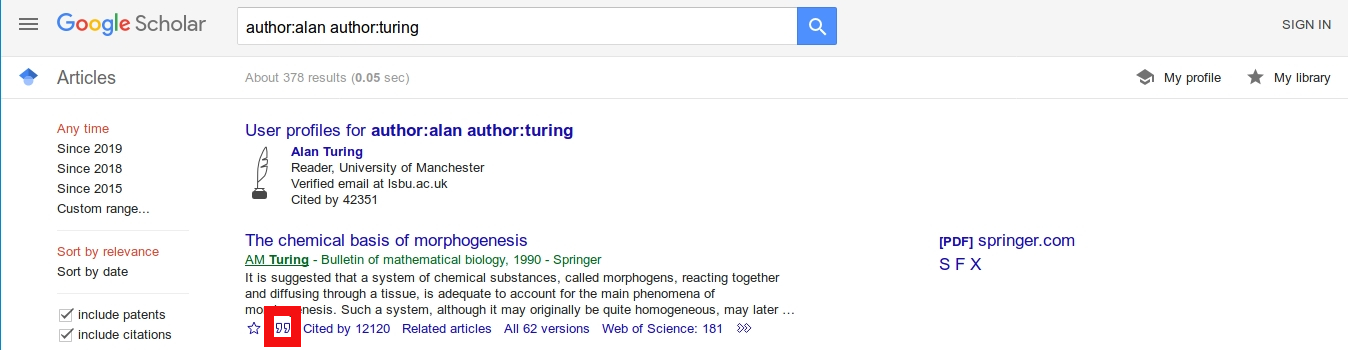
\includegraphics[width=\textwidth]{graphics/google_bibtex1.jpg}  
  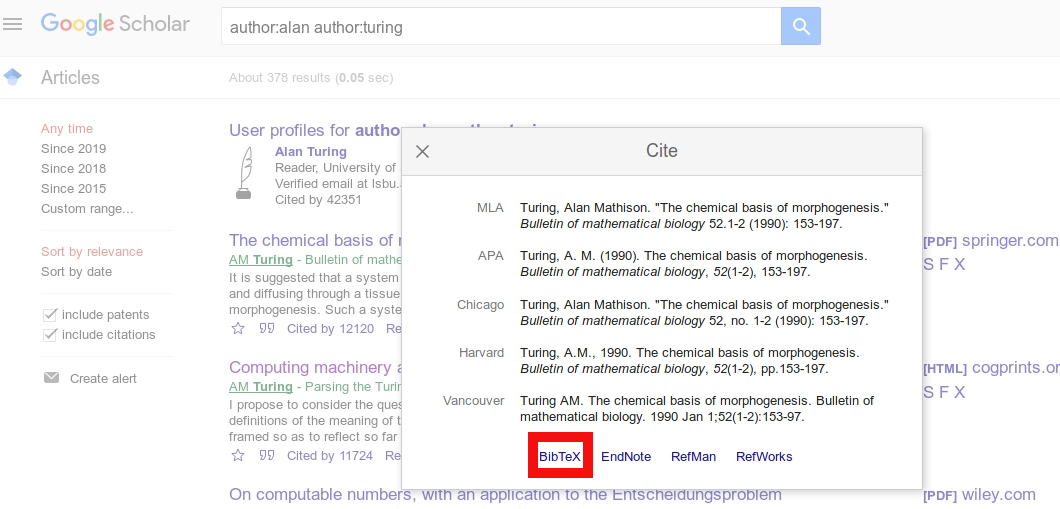
\includegraphics[width=\textwidth]{graphics/google_bibtex2.jpg}  
  \caption{Loading Bib\TeX{} entries from Google Scholar}
  \label{fig:google-scholar-bibtex}
\end{figure}

\section{Citing}
Bib\TeX{} extends \LaTeX{} by several commands (cf. \cref{tbl:bibtex-commands}). 
Make sure to include the \mintinline{sh}{natbib} package for this purpose.

\begin{table}[H]
  \centering
  \begin{tabular}{ll}
  \toprule
  Function                 & Command \\ \midrule
  Citing sources           & \mintinline{latex}{\cite{<source>}} \\
  Citing pages             & \mintinline{latex}{\cite[p. 15]{<source>}} \\
  Custom citations         & \mintinline{latex}{\cite[<prefix>][<suffix>]{<source>}} \\
  Including the bibliography     & \mintinline{latex}{\bibliography{<bibliographyfile>}} \\
  Setting the bibliography style & \mintinline{latex}{\bibliographystyle{<style>}} \\ \bottomrule
  \end{tabular}
  \caption{Commands for citations}
  \label{tbl:bibtex-commands}
\end{table}

The \mintinline{latex}{<source>} of a citation is always a Bib\TeX{} key.
The list of available citation styles\footnote{Head to Overleaf for a rather complete list: \url{https://www.overleaf.com/learn/latex/Biblatex_citation_styles}} includes alpha, natdin, and apa.
The table of references will always appear where the \mintinline{latex}{\bibliography{…}} command was put.
The \mintinline{latex}{\cite} command comes with many variants.\footnote{cf. \url{https://www.economics.utoronto.ca/osborne/latex/BIBTEX.HTM}}

\Example{lst:natdin-example}{literature/natdin-example}{literature/natdin-example_bib}{Exemplary citations in the \mintinline{latex}{natdin} style.}

\chapter{Prospects}
\label{sec:prospects}

Obviously, in this script, we were not able to show you the least of what \LaTeX{} has to offer. 
Therefore, in this last section, we gathered some information to help you to go further into depth by yourself.

\section{Packages}

We already have presented a selection of packages. However, there are thousands more of them. In the following sections we have put together some packages for frequently needed features: 

\begin{figure}[p]
	\widebox{
		% Top rules:
		\colrules
		% Left content: code listing:
		\begin{subfigure}{\widefigurewidth}
			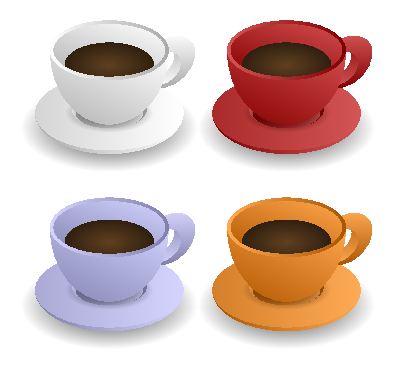
\includegraphics[width=\linewidth]{graphics/coffee-cup.pdf}
		\end{subfigure}
		\hspace{\widefiguregap}
		% Right content: image or rendered example:
		\begin{subfigure}{\widefigurewidth}
			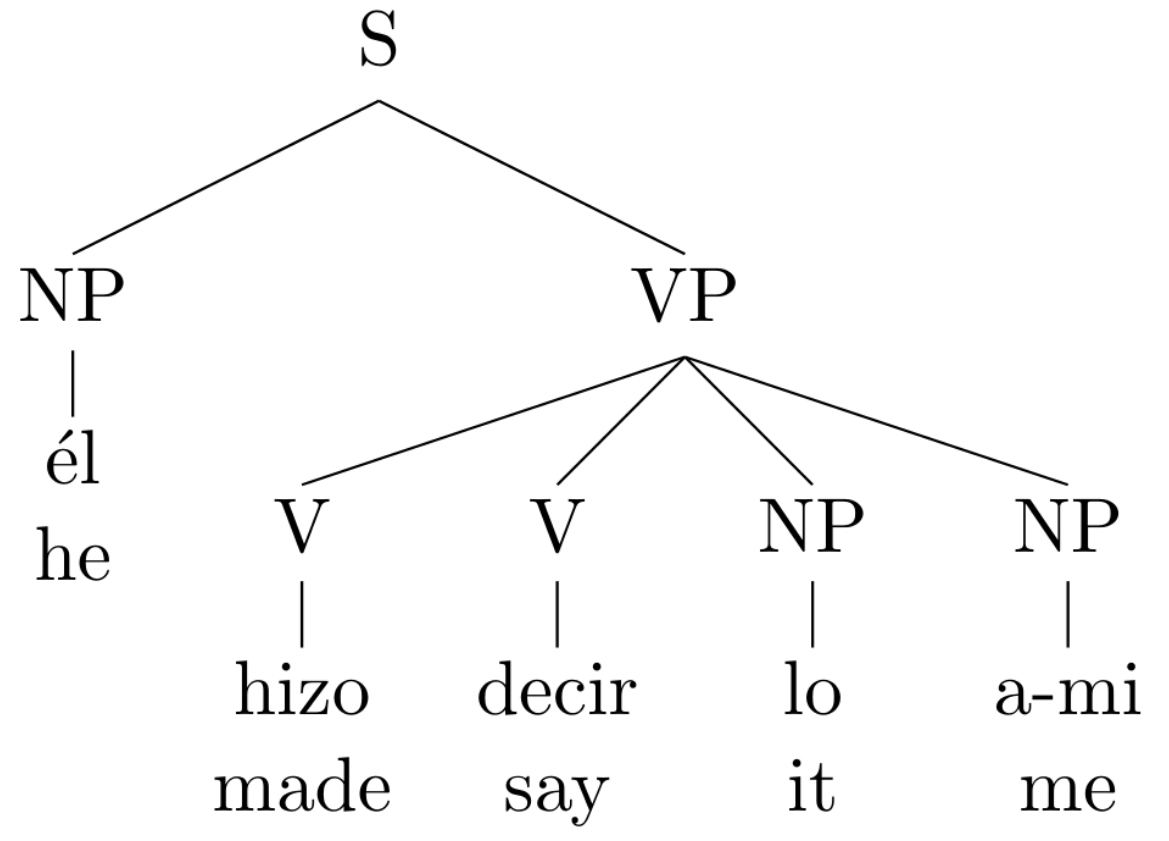
\includegraphics[width=\linewidth]{graphics/qtree.png}
		\end{subfigure}
		% Bottom rules:
		\colrules
		% Left caption:
		\begin{subfigure}[t]{\widefigurewidth}
			\caption{Vector graphics with TikZ}
			\centering\tiny{\url{https://texample.net/tikz/examples/coffee-cup/}}
			\label{fig:tikz-example}
		\end{subfigure}
		\hspace{\widefiguregap}
		% Right caption:
		\begin{subfigure}[t]{\widefigurewidth}
			\caption{Parse trees with qtree}
			\centering\tiny{\url{https://www.ling.upenn.edu/advice/latex/qtree/}}
			\label{fig:qtree-example}
		\end{subfigure}
		\medskip

		% Top rules:
		\colrules
		% Left content: code listing:
		\begin{subfigure}{\widefigurewidth}
			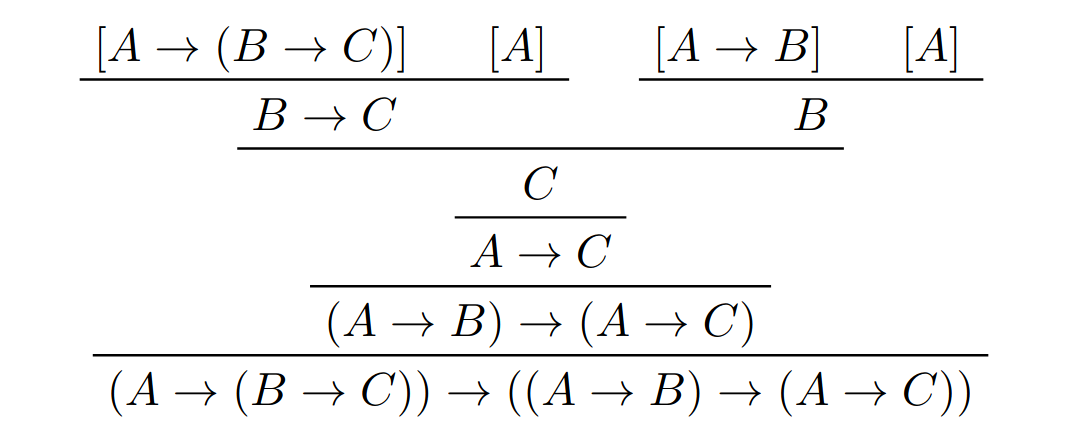
\includegraphics[width=\linewidth]{graphics/prftree.png}
		\end{subfigure}
		\hspace{\widefiguregap}
		% Right content: image or rendered example:
		\begin{subfigure}{\widefigurewidth}
			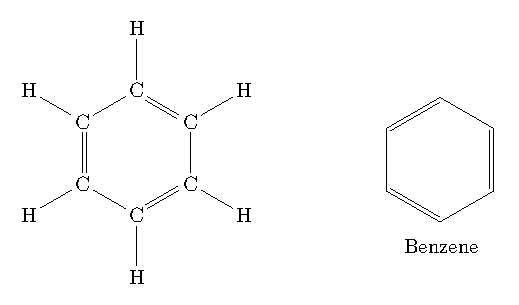
\includegraphics[width=\linewidth]{graphics/benzene-ring.pdf}
		\end{subfigure}
		% Bottom rules:
		\colrules
		% Left caption:
		\begin{subfigure}[t]{\widefigurewidth}
			\caption{Proof trees with prftree}
			\centering\tiny{\url{https://ftp.gwdg.de/pub/ctan/macros/latex/contrib/prftree/}}
			\label{fig:prftree-example}
		\end{subfigure}
		\hspace{\widefiguregap}
		% Right caption:
		\begin{subfigure}[t]{\widefigurewidth}
			\caption{Chemical structural formulas with chemfig}
			\centering\tiny{\url{http://latex-cookbook.net/cookbook/examples/benzene-ring/}}
			\label{fig:chemfig-example}
		\end{subfigure}
		\medskip
	}
	% General caption:
	\caption{Examples for some packages}
	\label{fig:package-examples}
\end{figure}


\begin{description}
	\item[Indices]
		can be created automatically with \texttt{makeidx}.\footnote{\url{https://www.ctan.org/pkg/makeidx}}
		By using \mintinline{tex}{\index{…}}, one can mark entries for the index. With \mintinline{tex}{\printindex}, \replaced[id=C]{an index with references is compiled out of them}{they are assembled within index with references}.
	\item[Vector graphics]
		(\cref{fig:tikz-example})
				can be \enquote{drawn} directly in the \LaTeX{} source code with \texttt{TikZ} (recursive acronym for \emph{TikZ ist kein Zeichenprogramm}, in English: \emph{TikZ is not a drawing program}).\footnote{\url{https://www.ctan.org/pkg/pgf}}
		Caution: This package is very powerful, but not necessarily beginner-friendly.
		Before creating vector graphics from sratch, we recommend you to experiment with some of the examples at \TeX{}ample\footnote{\url{https://texample.net/tikz/examples/}}. 
		\replaced[id=C]{Also, f}{F}or certain use cases, there are special packages that are easier to handle than \enquote{raw} TikZ:
	\item[Parse trees]
		that divide sentences into their grammatical components (\cref{fig:qtree-example}) can be created with \texttt{qtree}.\footnote{\url{https://ctan.org/pkg/qtree}}
	\item[Proof trees,]
		that are often used in logics (\cref{fig:prftree-example}), can be drawn with the package \texttt{prftree}.\footnote{\url{https://www.ctan.org/pkg/prftree}}
	\item[Chemical structural formulas]
		(\cref{fig:chemfig-example})
		can, amongst others, be created with  \texttt{chemfig}.\footnote{\url{https://www.ctan.org/pkg/chemfig}}
	\item[Colors]
		for your documents are provided by \texttt{xcolor}.\footnote{\url{https://www.ctan.org/pkg/xcolor}}
	\item[Note]
		\deleted[id=C]{that you have made in your source code and} that you cannot overlook can be created with \texttt{todonotes}.\footnote{\url{https://www.ctan.org/pkg/todonotes}}
		With the package, \replaced[id=C]{you}{one} can mark what \replaced[id=C]{you}{they} still \todo{Please do not change. This is an example.} have to change within \replaced[id=C]{your}{their} document.
	\item[Pages of other \acro{PDF} files]
		can be integrated into the source code with \texttt{pdfpages}.\footnote{\url{https://www.ctan.org/pkg/pdfpages}}
		It comes in very handy whenever one needs the output of external programs in the document, for example, in\deleted[id=C]{ within} within the appendix.
		Just compile the document one more time and the appendix is up-to-date again, if the external program has changed something.
	\item[Nested graphics]
		and the positioning of captions at almost any place are provided by  
		\texttt{subcaption}.\footnote{\url{https://www.ctan.org/pkg/subcaption}}
		We also made extensive use of this package.
	\item[Tables]
		can be designed much more flexibl\replaced[id=C]{y}{e} than what we have shown here. 
		The following packages can help you with that:
		\texttt{colortbl},\footnote{\url{https://www.ctan.org/pkg/colortbl}}
		\texttt{tabularx},\footnote{\url{https://www.ctan.org/pkg/tabularx}}
		\texttt{multirow},\footnote{\url{https://www.ctan.org/pkg/multirow}}
		\texttt{makecell}.\footnote{\url{https://www.ctan.org/pkg/makecell}}
\end{description}

\noindent \texttt{beamer}, which is not a package, but another document class, can be used to create \textbf{slide shows}
with \LaTeX{}. Information on the document class and examples are available at Overleaf,\footnote{\url{https://www.overleaf.com/learn/latex/Beamer}} which brings us to the next section:

\section{Help and information}

\textbf{Wikibooks} provides you with a much more detailed introduction into \LaTeX{}. Note that the German version\footnote{\url{https://de.wikibooks.org/wiki/LaTeX-Kompendium}} is less complete than the English one.\footnote{\url{https://en.wikibooks.org/wiki/LaTeX}}
If required, both refer to additional packages.

Whenever you need information on certain packages, \acro{\textbf{CTAN}}\footnote{\url{https://ctan.org/}} is your place to go. 
\replaced[id=C]{For each package, you can find the official documentation as a \acro{PDF} file there.}{The official documentation as \acro{PDF} for each package can be found there.}
Within this file, the first paragraphs are \added[id=C]{usually }the most interesting. They are 
followed by implementation details, that you normally do not need.

If the official documentation is too theoretical, and you prefer a more hands-on approach, \textbf{Overleaf}\footnote{\url{https://www.overleaf.com/}} can help you out.
Primarily, it is a collaborative online \LaTeX{} editor. However, you can find multiple templates\footnote{\url{https://www.overleaf.com/latex/templates}} for different types of documents (VCs, theses, \textellipsis) there.

If you are looking for examples dedicated to TikZ, \textbf{\TeX{}ample}\footnote{\url{https://texample.net/}} provides you with multiple of them.

For concrete questions, the question-answering platform \textbf{Stackexchange} is a good place to go: There even is a \TeX{} community there.\footnote{\url{https://tex.stackexchange.com/}}

\replaced[id=C]{Of course}{Needless to say}, you can always contact us with your questions:
\begin{compactitem}
	\item via mail to \href{mailto:fachschaft-wiai.stuve@uni-bamberg.de}{fachschaft-wiai.stuve@uni-bamberg.de},
	\item via phone at +49951\,863\,1219,
	\item or just come to our bureau at WE5/02.104.
\end{compactitem}




% References

\end{document}
